% Or call it Research results?

\chapter{Evaluation}
\label{chap:evaluation}
This chapter presents the experiments and results that have been conducted. The data and language modeling process needed for all of the experiments is presented in the first two sections, respectively. Then, the experiments are presented one by one. 

The experiments are grouped by research question. Experiment \textbf{E1} takes on research question 1 regarding automatic smart contract code synthesis. Expand to \textbf{E1.1} and \textbf{E1.2}It explores the performance of a pre-trained transformer-based language model on the verified smart contract dataset. Experiment \textbf{E2} focuses on the security of smart contract code generation, tackling research question 2. It compares the security of a fine-tuned model utilizing security conditioning purposed in \cref{sec:security-conditioning}. This section presents three sub-experiments:
\begin{enumerate}[label=\textbf{E2.\arabic*.}, leftmargin=1.5cm]
    \item Compares security performance based on providing entire class context from audited verified smart contract dataset.
    \item Compares security performance based on using only comments as input context from audited verified smart contract dataset.
    \item Compares security performance based on testing a custom vulnerability-inclined dataset.
\end{enumerate}
The last experiment \textbf{E3} takes on research question 3 regarding how to best formulate the input for automatic smart contract code synthesis.

\section{Evaluation of RQ1}
\label{sec:e1-automatic-smart-contract-code-synthesis}
This section evaluates the performance of the implementation developed for research question 1. Describe different scenarios  (contexts), full and comment only. 

\subsection{Evaluation metrics}
Using bleu score in abscence of something better.


\subsection{Code context}
\subsection{Comment context}
=> This leads

\subsection{Full context}

\subsection{Transfer learning}
Until now, the focus has been on Solidity. However, the training data also contains a very small amount of Vyper code. 

\subsection{Pre-trained model}
\label{sec:eval-pre-trained-model}
The pre-trained model is used to generate code for a smart contract. This shows wether such mudels are able to generate code for a smart contracts, even thoug they are trained on a very limited set of smart contract code. This serves to answer research  question 1.1. This also serves as the baseline for comparison in experiment E1.2

Use the pre-trained GPT-J-6B model from ElutherAI, as described in \cref{sec:pretraining}.

Report accuracy?


\section{Evaluation of RQ2}
How secure is the generated code?

\subsection{Inclined Vulnerabilities}
\label{sec:inclined-vulnerabilities}

Evaluation dataset.


\subsection{E1.1 - Fine-tuned model}
\label{sec:e2.1-fine-tuned-model}

\subsubsection{Method and Data}
\subsubsection{Results and Discussion}


\begin{figure}[htp]
    \centering
    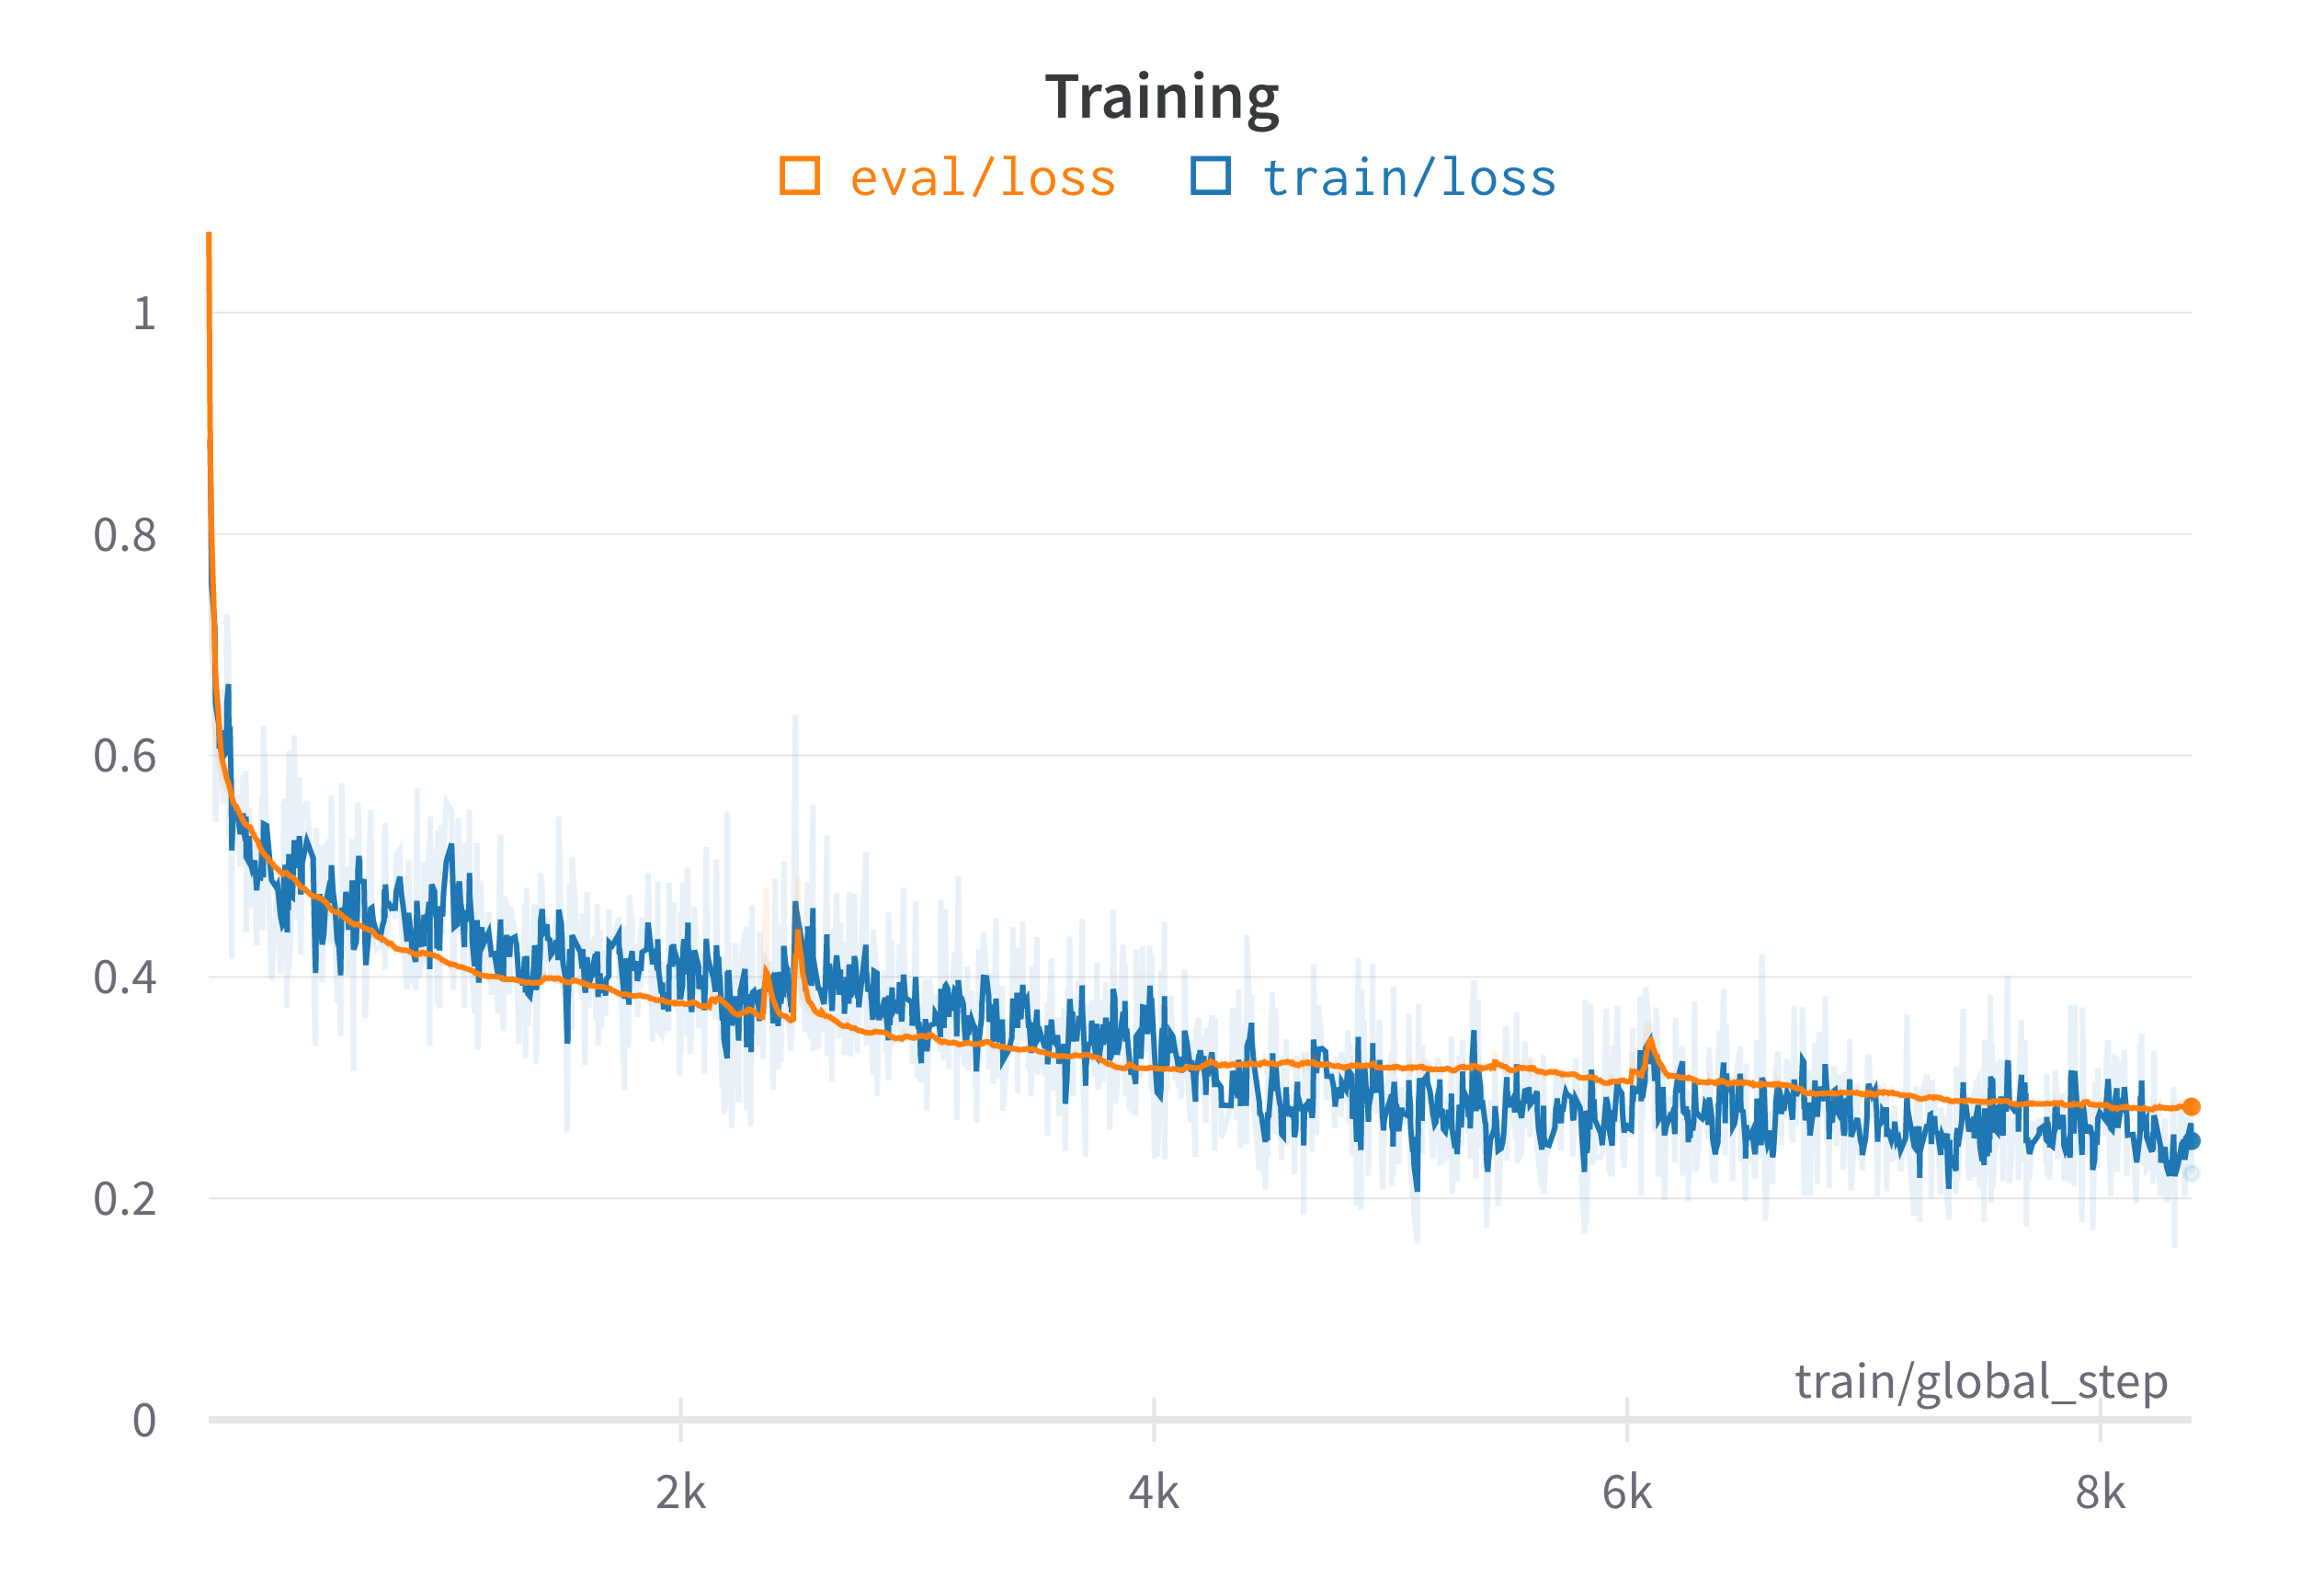
\includegraphics[width=\textwidth]{figures/wandb-train-loss-gpt-j-smart-contract.png}
    \caption{Training and evaluation loss during model training.}
\end{figure}

\begin{figure}[htp]
    \centering
    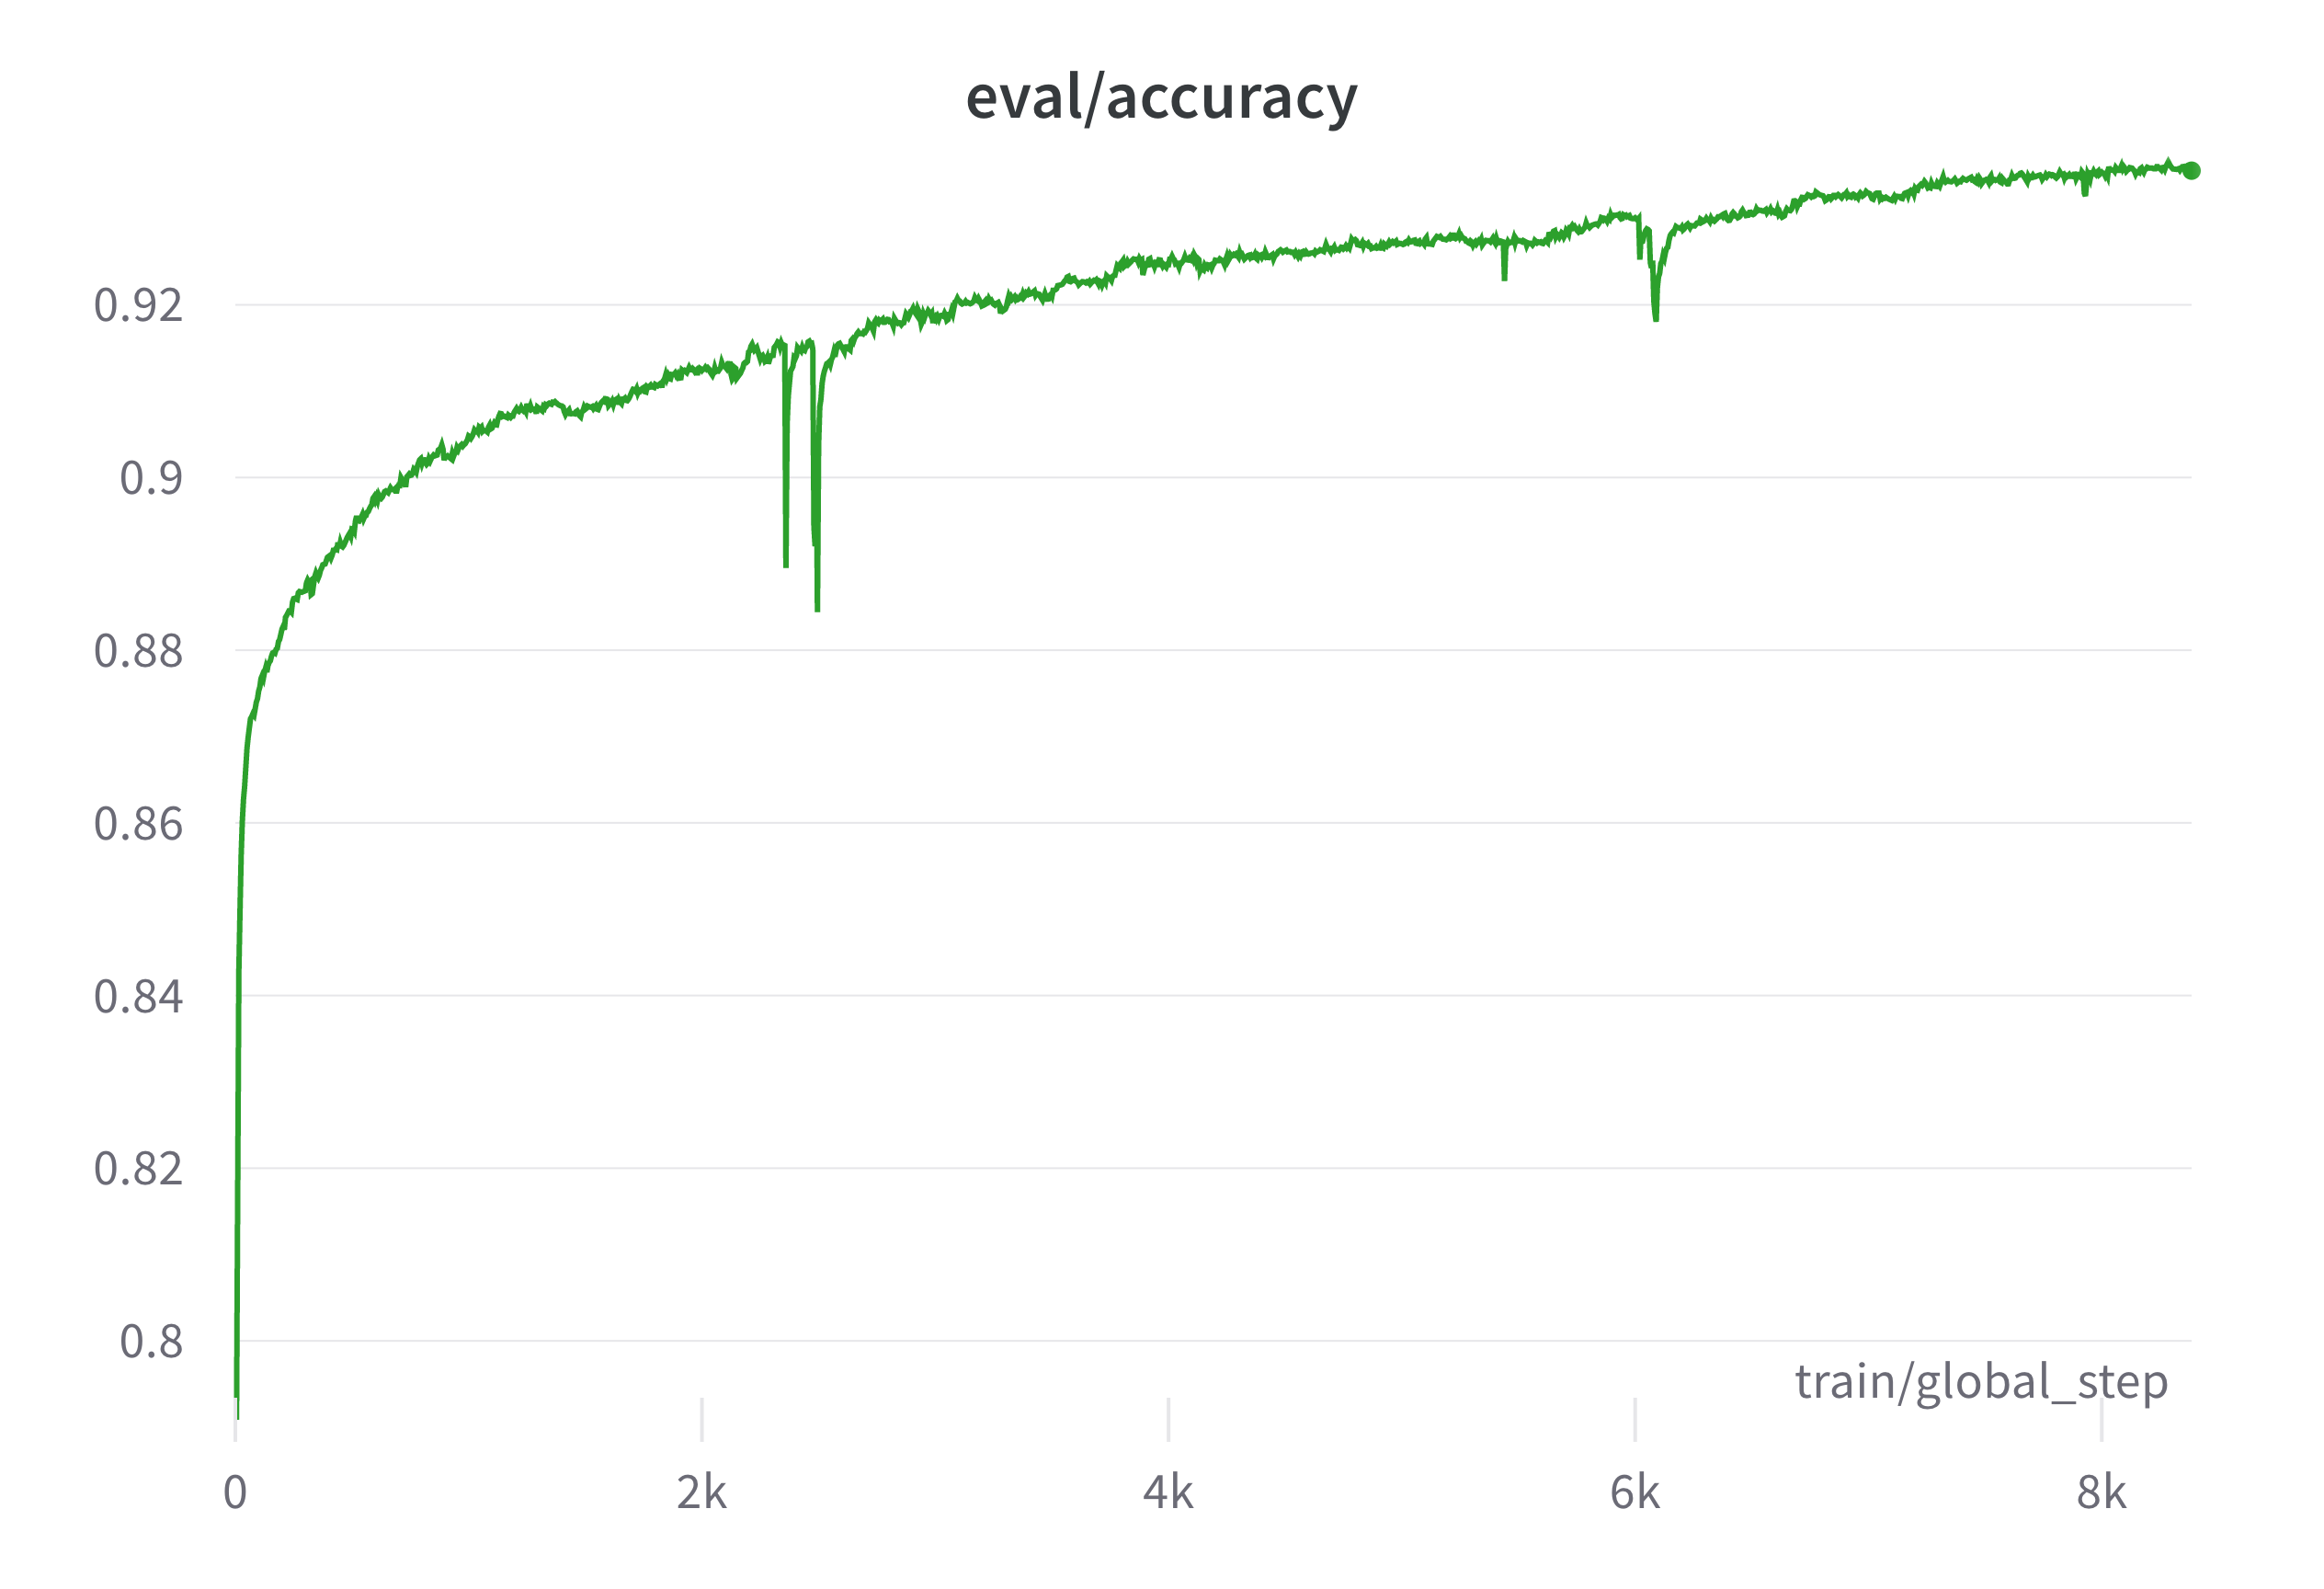
\includegraphics[width=\textwidth]{figures/wandb-train-eval-gpt-j-smart-contract.png}
    \caption{Evaluation accuracy during model training.}
\end{figure}


\section{E2 - Security Conditioning}
\label{sec:e2-security-conditioning}
This section presents the results and discussion of the sub-experiments of experiment \textbf{E2}. Experiment \textbf{E2} focuses on the security of smart contract code generation, tackling research question 2. It compares the security of a fine-tuned model with and without utilizing security conditioning purposed in \cref{sec:security-conditioning}. The following three sub-experiments are all based on the same fine-tuned models, but uses different evaluation method.

\subsubsection{Method and Data}
Using security conditioning reduces the frequency of vulnerable code.

\subsubsection{Results and Discussion}
Include attenttion weightts of the model. And training results.

\label{sec:e2.1-complete-class-context}

\subsubsection{Method and Data}
\subsubsection{Results and Discussion}

No significant difference between the two models. In fact, it seems to be worse. ... It is, therefore, reasonable to hypothesize that this is due to the limited sample space available. The existing contract code provided as input context could be biased. This motivates the use of a smaller input context. This should increase the sample space and allow the model to make better use of the security conditioning. This hypothesis is the basis for Experiment E2.2.

\subsection{E2.2 - Comment Context}
\label{sec:e2.2-comment-context}

\subsubsection{Method and Data}

\subsubsection{Results and Discussion}
Still, no significant differences can be observed. Upon further inspection of the generated code (qualitative), most of the reported vulnerabilities are due to the generation of classes instead of functions. Another problem seems to be that the vulnerability detection tool is not able to detect the vulnerabilities in the generated code. Since the generated code is primarily confined to only one function, potential problematic code such as integer overflow needs an actual state variable in order to be classified as a vulnerability. Since this is not possible, it motivated the creation of a tailor-made evaluation dataset, and is the basis for Experiment E2.2.


\subsection{E2.3 - Inclined Vulnerabilities}
\label{sec:e2.3-inclined-vulnerabilities}
By using a custom made evaluation dataset, it can be hypotthesized that this more accurately capttures the behaviour of the system as it would be used in production.

\subsubsection{Method and Data}
For this experiment, a tailor-made evaluation dataset was created for the sole purpose of evaluating how secure the model is. The dataset is described in detail in \cref{sec:inclined-vulnerabilities}

\subsubsection{Results and Discussion}
Hopefully good results!!! If so, do statistical hypothesis testing to investigate the significance of the observation.

\textbf{\(H_0\)}: A model using security conditioning does not produce fewer vulnerabilities. 
\textbf{\(H_1\)}: A model using security conditioning produces fewer vulnerabilities.


\section{E3 - Formulation of Inputs}
\label{sec:e3-formulation-of-inputs}
For answering research question 3, this experiment focuses on the formulation of inputs to the model. Specifically, it investigates how comments can be constructed and formatted in order to generate the best possible code.

\subsubsection{Method and Data}
Clustering of data from verified smart contracts dataset. Elaborate... Select based on elbow method. From the clustered results, 10.000 random samples are selected from each of the clusters. These samples are used to generate code. The function's comment and the function's signature are used as input to the fine-tuned models. One with security conditioning and one withou. The results are then compared.

\subsubsection{Results and Discussion}






\section{Summary}






\todo{Move to datasets?)}
\section{InclinedVulnerabilities}

Custom dataset containing multiple hand written INCOMPLETE contracts that MAY produce vulnerabilities.


\todo{Move relevant stuff below to method chapter (experiment plan)}
\section{Baselines}
\subsection{InclinedVulnerabilities}

\section{Evaluation metrics}
\todo{Rewrite}
Accuracy could measure correctness of the exact match, failing, however, to capture the proximity when a completion suggestion partially matches the target sequence, which could still be a valid completion suggestion.

\todo{Rewrite}
The ROUGE score is the metric commonly used to evaluate machine translation models. Its ROUGE-L variant is based on the Longest Common Subsequence (LCS) statistics. LCS takes into account structure similarity and identifies longest co-occurring n-grams.

\todo{Rewrite}
The Levenshtein distance measures how many single-character edits  including insertion, substitution, or deletion - does it take to transform one sequence of tokens to another. Quite often, even if a suggested completion is only an approximate match, developers are willing to accept it, making appropriate edits afterwards. As such, the Levenshtein edit similarity is a critical evaluation metric.


Get logits from a model  prediction to visualize the distribution of the predicted probabilities.

\section{Quantitative evaluation}

Even though only "HIH" severity vulnerabilities are labeled, several most of these also contain medium and low severity vulnerabilities. See Doughnut chart...  
The "full" context code is subject to latent vulnerabilities, which are unavoidable. Hence this could explain the low decrease in vulnerabilities.




\section{Qualitative evaluation}


\section{Memorisation evaluation}
Check if the model is just copying

Do this by investigating logits from  all layers.

Check common substrings in dattaset.

\section{Diff}

Tryto make custom generattion function that only selects SECURE solutions.....??

Does the temperature affect how secure solutions are?


Huugging face emojie as transformer model!


\section{Model weigts}
THIS USES AN INDUCTIVE ANALYSIS. Fix methodology chapter. ADD as Experiment 4?

Can  we  find structures in the eriht? Neural  view? bertviz? That resembles AST equivalent?

Answers to research questions
Evaluation of the answers